\chapter{Manual de usuario}

En este apéndice se pretende hacer conocer al usuario final del software cómo se maneja el mismo. Con un sencillo ejemplo de utilización quedarán claros los diferentes apartados de la interfaz.
\bigskip

\section{Ejemplo de uso}

Para comenzar a utilizar por primera vez la interfaz gráfica de Big Data para MEDA-Toolbox se debe tener previamente un fichero índice con las rutas a todos los ficheros a analizar como se vio en el capítulo 8. La estructura de los ficheros de datos debe seguir los patrones explicados en el mismo capítulo.

\bigskip

\begin{figure}
\centering
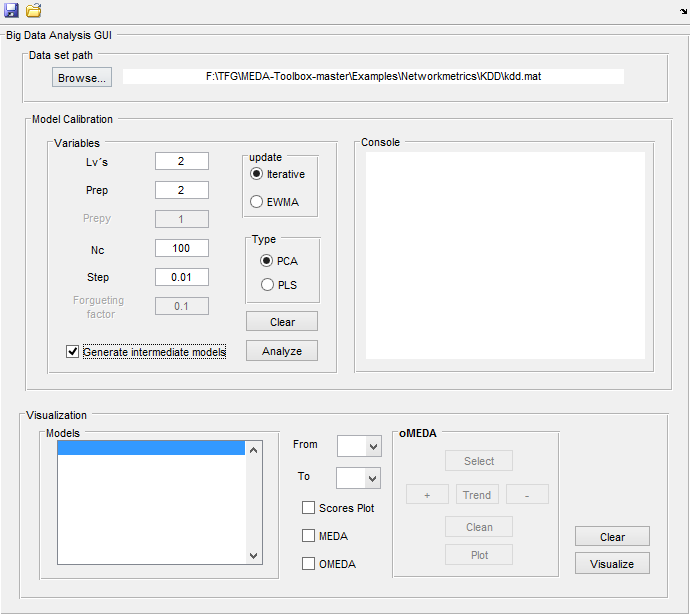
\includegraphics[width=0.8\textwidth]{imagenes/figuras/MU-1.png}
\caption{MEDA-Toolbox BIG DATA GUI.}
\end{figure}

Una vez se tienen correctamente los ficheros de datos y el índice se pasa a cargar los datos en el entorno, esto se hace pulsando el botón "Browse" de la sección "Data set path", esto producirá la apertura de un interfaz de selección de archivos, como el de la figura A-2.

\bigskip

\begin{figure}
\centering
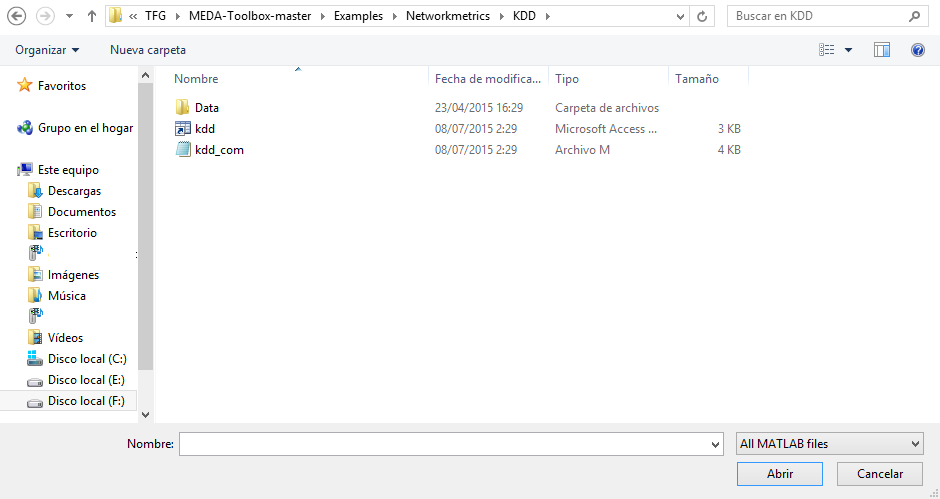
\includegraphics[width=0.8\textwidth]{imagenes/figuras/MU-2.png}
\caption{Interfaz de selección de ficheros.}
\end{figure}

\bigskip

En este caso se ha seleccionado el fichero \textbf{kdd.mat} del ejemplo de \textbf{Networkmetrics} de MEDA-Toolbox. Ya marcado el fichero se le da al botón \textbf{Abrir} cargando así los datos del mismo en el entorno de Matlab.

\bigskip

Cada uno de los campos de la sección \textbf{Variables} se explicó en el capítulo 8, por lo que en este apéndice no se va a comentar nada nuevo al respecto, únicamente se va a proseguir con el ejemplo con los valores por defecto.

\bigskip

Si se desea realizar un análisis iterativo utilizando \textbf{PCA} se deben marcar las casillas correspondientes de las subsecciones \textbf{Update} y \textbf{Type} como se puede apreciar en la Figura A.1. Para generar un modelo por cada fichero se debe marcar la casilla \textbf{Generate intermediate models}.

\bigskip

Durante la ejecución del análisis se puede ver en la sección \textbf{Console} las salidas que produce el software, como se puede observar en la figura A.3.

\begin{figure}
\centering
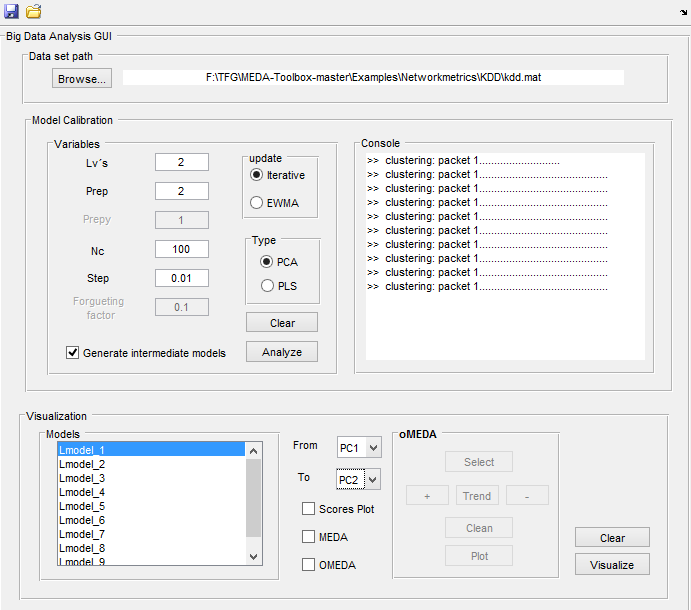
\includegraphics[width=0.8\textwidth]{imagenes/figuras/MU-3.png}
\caption{Interfaz con salidas del análisis.}
\end{figure}

\bigskip

Una vez realizado el análisis y la calibración del modelo se pasa a la visualización para la cual tenemos 3 tipos de gráficos. Se comenzará seleccionando \textbf{ScorePlot} y/o \textbf{MEDA} y tras generar el Score Plot se creará el \textbf{oMEDA}, ya que este último depende de que ya este generado el mismo para poder seleccionar de el los puntos que se deseen plotear en oMEDA.

\bigskip

Para que se muestren los gráficos debemos pulsar \textbf{Visualize}, no sin antes seleccionar de la lista \textbf{From} el valor del primer componente principal desde el que comenzar la visualización y en \textbf{To} el último componente, generándose los gráficos Score Plots comparando todos los PCs intermedios entre los dos seleccionados, incluyéndose ambos en la comparación.

\bigskip

La figura A.4 es el ScorePlot del modelo y la A.5 es el gráfico MEDA.

\begin{figure}
\centering
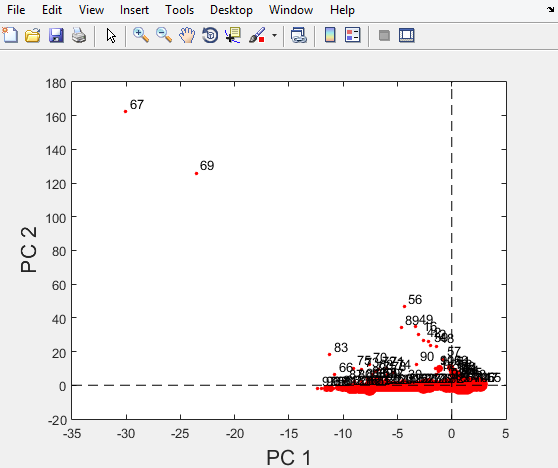
\includegraphics[width=0.8\textwidth]{imagenes/figuras/MU-4.png}
\caption{Score Plot del ejemplo.}
\end{figure}

\begin{figure}
\centering
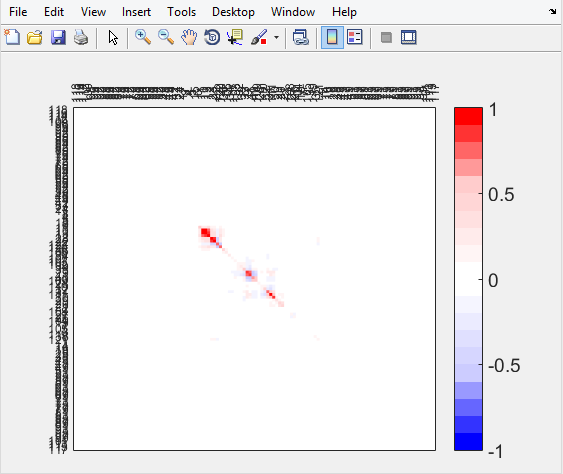
\includegraphics[width=0.8\textwidth]{imagenes/figuras/MU-5.png}
\caption{MEDA del ejemplo.}
\end{figure}

\bigskip

Por último para generar el gráfico oMEDA se marca la casilla de mismo nombre, lo que activará la sección con las herramientas necesarias para poder llevar a cabo el gráfico.

\bigskip

Una vez activado el menú oMEDA y con un ScorePlot abierto se le da al botón \textbf{Select} lo que traerá a primer plano el mismo para que se seleccionen los puntos, esto se ve en la figura A.6. En dicha figura se pueden ver los puntos en blanco lo que ocurre cuando tras hacer el polígono pulsamos el botón \textbf{mas}.

\begin{figure}
\centering
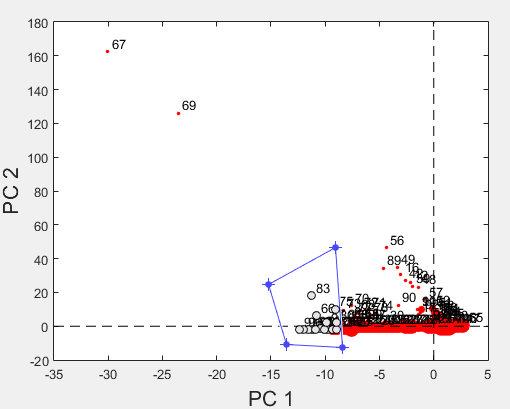
\includegraphics[width=0.8\textwidth]{imagenes/figuras/MU-6.png}
\caption{Selección de puntos en un ScorePlot.}
\end{figure}

\begin{figure}[H]
\centering
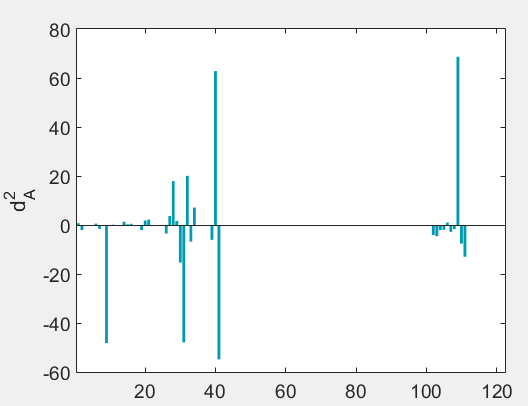
\includegraphics[width=0.8\textwidth]{imagenes/figuras/MU-7.png}
\caption{Gráfico oMEDA del ejemplo.}
\end{figure}

Ahora que ya se tienen los puntos pulsamos el botón \textbf{plot} y se mostrará la gráfica oMEDA de la figura A.7.

\bigskip

\section{Fallos comunes}

En esta sección se van a comentar los mensajes de error y posibles problemas que puede producir la aplicación en su uso.

\subsection{Mensajes de error}

El primer mensaje de error que se da cuando se intenta comenzar un análisis sin que exista un fichero seleccionado, como se ve en la figura A.8.

\begin{figure}[H]
\centering

\includegraphics[width=0.8\textwidth]{imagenes/figuras/MU-8.png}
\caption{Mensaje de error de fichero.}
\end{figure}


Para cada uno de los campos del apartado Variables, hay un mensaje de error cuando no se rellenan, los mensajes son del tipo de la figura A.9.

\begin{figure}[H]
\centering
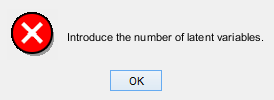
\includegraphics[width=0.8\textwidth]{imagenes/figuras/MU-9.png}
\caption{Mensaje de error de campo sin rellenar.}
\end{figure}


Otro mensaje de error es generado cuando en el apartado de Visualization los campos From y To tienen el mismo valor, lo cuál hace que no se pueda mostrar la visualización y muestra un mensaje como el de la figura A.9.

\begin{figure}
\centering
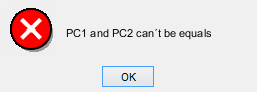
\includegraphics[width=0.8\textwidth]{imagenes/figuras/MU-10.png}
\caption{Ejemplo mensaje de error PCs iguales.}
\end{figure}

\subsection{Problemas típicos}

Los problemas que pueden ocurrir a la hora de ejecutar la aplicación normalmente se dan por no tener incluidas la toolbox o la interfaz big data dentro del path de matlab, esto se puede ver en la figura A.11.


\begin{figure}[H]
\centering
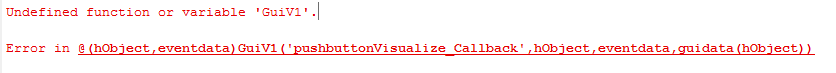
\includegraphics[width=0.8\textwidth]{imagenes/figuras/MU-11.png}
\caption{Matlab no reconoce la GUI.}
\end{figure}

Esto se soluciona agregando los ficheros de la GUI a Matlab, se puede hacer de varias formas, de manera definitiva en la pestaña \textbf{Home} de matlab en el botón \textbf{Set path}, o cada vez que se vaya a ejecutar la aplicación, paraece un mensaje como el de la figura A.12 y pulsando sobre \textbf{Add to Path} lo agrega para esa sesión.

\begin{figure}[H]
\centering
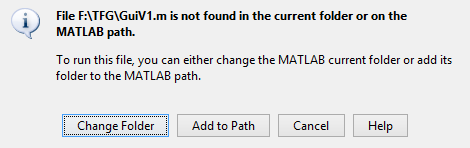
\includegraphics[width=0.8\textwidth]{imagenes/figuras/MU-12.png}
\caption{Mensaje de inicio de GUI.}
\end{figure}

